\documentclass[11pt]{standalone}
\usepackage{pgf, tikz}
\usetikzlibrary{arrows, automata}

\begin{document}
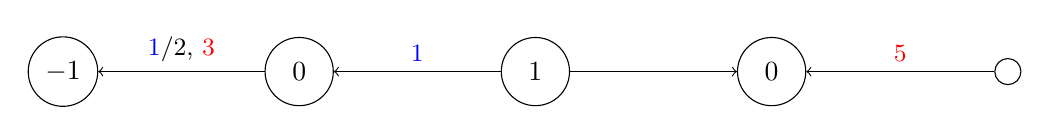
\begin{tikzpicture} [align=center]
\path (0, 0) node[circle, draw, text width=0.5cm] (v0) {$-1$}
      (3, 0) node[circle, draw, text width=0.5cm] (v1) {$0$}
      (6, 0) node[circle, draw, text width=0.5cm] (v2) {$1$}
      (9, 0) node[circle, draw, text width=0.5cm] (v3) {$0$}
      (12, 0) node[circle, draw] (v4) {};
      
\draw[<-] (v0) to node [above] {\small \textcolor{blue}{1}/2, \textcolor{red}{3}} (v1);
\draw[<-] (v1) to node [blue, above] {\small 1}(v2);
\draw[->] (v2) to (v3);
\draw[<-] (v3) to node [red, above] {\small 5}  (v4);

\end{tikzpicture}
\end{document}